\chapter{A mechanized framework for reasoning on software architectures}
\chaptermark{Mefresa}
\label{chap:mefresa} 
\epigraph{\textit{“If I had asked people what they wanted, they would have said faster horses.”}}{Henry Ford}
	
\minitoc

\lhead{Chapter 1. \emph{Mefresa}} % This is for the header on each page - perhaps a shortened title
	
This chapter presents \textsc{Mefresa} (\textit{\textbf{Me}chanized \textbf{F}ramework for \textbf{Re}asoning on \textbf{S}oftware \textbf{A}rchitectures}), a Coq framework for reasoning on software architectures.
	It focuses on the \ac{GCM}, detailing how its specificities were mechanized in a proof assistant like Coq. 
	Moreover, a simple \textsf{operation} language is proposed for the safe composition of 
	\ac{GCM} architectures. Concrete examples complete its presentation.
		
	The results discussed in this chapter were partially published as a \textit{short paper} at the proceedings
	of the \textit{Conf\'erence en Ing\'enieriE du Logiciel} (CIEL'2012) \cite{gaspar:hal-00725291} held
	at the \textit{Universit\'e de Rennes},
	and at the \textit{International Journal of Parallel Programming} as a special issue
	of the \textit{International Symposium on High-level Parallel Programming and Applications} (HLPP'2013) \cite{GASHENMAD:IJPP13},
	held at the \textit{Institut Henri Poincar\'e}, Paris.	
	
	Section \ref{sec:coqgcm} discusses the mechanization of the \ac{GCM} with the Coq
	proof assistant. In particular, we show how we use inductive definitions to model
	the \ac{GCM} core elements, and predicates to formally specify their structure
	and \textit{typing} requisites.
	A language for conveniently manipulating \ac{GCM} architectures
	is presented in Section \ref{sec:op}. Examples on mechanically proven properties
	are illustrated in Section \ref{sub:ex}.	For last, Section \ref{sec:mesfresadiscussion} gives
	some final remarks about this development.
	 
		
	For more details and release announcements of \textsc{Mefresa} 
	the interested reader is pointed to the website\footnote{\textsc{Mefresa}  is available online at: 
	\url{http://www-sop.inria.fr/members/Nuno.Gaspar/Mefresa.php}} of its development. 
%----------------------------------------------------------------------------------------
%% @@@@@@@@@@@@
\section{Mechanizing GCM with the Coq proof assistant}
\label{sec:coqgcm}
		
	
		As discussed in Section \ref{sec:gcm}, the \ac{GCM} is an extension to 
		Fractal. Both component models have their specification written in natural language, 
	thus inherently ambiguous and open to interpretation. In fact, in \cite{MERLE:2008:INRIA-00338987:1}, 
	this liability has already been acknowledged by the people behind Fractal: \textit{"However, there are 
	aspects of the [Fractal] specification that remain decidedly insufficiently detailed or ambiguous"}. To this end,
	they attempt to \textit{"correct these deficiencies by developing a formal specification"} in 
	Alloy \cite{Jackson:2002:ALO:505145.505149}. 
	
		The same reasoning applies to our case, except that we rely on the Coq proof assistant \cite{09thecoq}.
	We take advantage of its high expressiveness and effective rationale to give a 
	precise semantics to the structure of \ac{GCM} applications, and provide the means to reason about its
	composition. Further, we are not limited to finite domains, we can define and 
	prove general properties about parametrized structures. 
			
		In the following we devote the remaining of this Section	 to detailing the mechanization
	of the \ac{GCM} with the Coq proof assistant.	
						
		
\subsection{Core elements}
\label{sub:core}

			The \ac{GCM} has three core elements: 
		components, interfaces and bindings. Their structure and the way they interact
		are naturally encoded by means of inductive definitions.
		
\subsubsection{Interface datatype}		
		
		
		The \textsf{interface} datatype is depicted by Listing \ref{lst:interface}.

	\lstinputlisting[language=Coq, stepnumber=1, caption=\textsf{interface} datatype, label=lst:interface]{listings/chapter4/interface.tex}


	\noindent It is characterized by an \textit{id} denoting its name, a \textit{signature} corresponding
	to its java interface \textit{classpath}, and a \textit{path} identifying its location in the component's hierarchy 
	(i.e. the component it belongs to). More precisely, these fields are specified as shown by Listing \ref{lst:idsigpath}.
	
	\lstinputlisting[language=Coq, stepnumber=1, 
	                        caption={\textsf{ident}, \textsf{signature} and \textsf{path} datatypes}, 
	                        label=lst:idsigpath]{listings/chapter4/path.tex}
	
	
	\noindent The only subtlety concerns the \textsf{path} field. It should be noted that \ac{GCM} is a 
	hierarchical component model, and since by introspection an interface is able to identify the component 
	it belongs to, a \textsf{path} identifying this component is necessary. Its definition (Line 5) is a list of 
	identifiers, where these identifiers indicate the components that need to be traversed in 
	the hierarchy to reach the component holding the interface.	
	
		The intended meaning of the remaining fields should pose no doubt. An interface is of internal or
	external \textit{visibility}, possess a client or server \textit{role}, is of functional or non-functional
	\textit{functionality}, contains an optional or mandatory \textit{contingency}, and its \textit{cardinality}
	is of singleton, multicast or gathercast nature.
	
		Listing \ref{lst:role} and Listing \ref{lst:cont} illustrate the \textsf{visibility}
		and \textsf{contingency} datatypes, respectively.
		
	\begin{figure}[H]
	\begin{minipage}[b]{0.4\linewidth} 
	\centering
	\lstinputlisting[language=Coq, caption=\textsf{role} datatype, frame=1rb, label=lst:role]{listings/chapter4/role.tex}
	\end{minipage}
	\hspace{0.05cm}
	\begin{minipage}[b]{0.55\linewidth} 
	\centering
	\lstinputlisting[language=Coq, caption=\textsf{contingency} datatype, stepnumber=0, frame=1rb, label=lst:cont]{listings/chapter4/contingency.tex}
	\end{minipage}
	\end{figure}	  			
				
		
	\noindent The remaining encodings are performed analogously.  Moreover, comparing these
	values of these datatypes requires the explicit definition of such a function. For instance,
	Listing \ref{lst:beqrole} depicts a boolean equality function for the \textsf{role} datatype values.
	
	
	\lstinputlisting[language=Coq, stepnumber=1, 
	                        caption={Boolean equality function for the \textsf{role} datatype values}, 
	                        label=lst:beqrole]{listings/chapter4/beqrole.tex}
	
	
	\noindent Basically, it is a rather simple function returning \textsf{true} if the two \textsf{role} values are
	equal, and \textsf{false} otherwise. The only doubt that may arise concerns the contents of line 8:
	it defines the infix operator \textsf{==} that can be conveniently used in place of
	\textsf{beq\_role}. As expected, other boolean equality functions and their respective 
	convenient notation are defined analogously for other datatypes.	
	
\subsubsection{Component datatype}

		Let us now look at the two remaining core elements, \textsf{component} and \textsf{binding}. 
	Listing \ref{lst:component} depicts the \textsf{component} datatype.   
		
	
		\lstinputlisting[language=Coq, stepnumber=1, 
	                        caption={\textsf{component} datatype}, 
	                        label=lst:component]{listings/chapter4/component.tex}

		\noindent A \textsf{component} also possesses an identifier and a \textsf{path} indicating its level in the hierarchy.
		As expected, its \textsf{implementationClass} field is a string holding the java class of its implementation.	
		Its \textsf{controlLevel} field determines its level of control: this feature however, is currently a mere 
		\textit{placeholder} with default value \textsf{Configuration}, 
		it is only kept for the sake of possible future enhancements. 
		A list of sub\textsf{component}s, a list of \textsf{interface}s and a list of \textsf{binding}s conclude its
		composition. 
		 
%%%%		 

			Before proceeding to the definition of \textsf{binding}s, let us discuss two auxiliary functions.
		A \textsf{component} is composed by several elements. It is therefore rather useful to
		make them easily accessible through \textit{projections}.	For instance, Listing \ref{lst:projid}
		depicts such a projection for the \textsf{component}'s \textsf{identifier} element.
							
		\lstinputlisting[language=Coq, stepnumber=1, 
	                        caption={Projection for the \textsf{component identifier} element}, 
	                        label=lst:projid]{listings/chapter4/projid.tex}

	\noindent Indeed, a simple pattern matching exposes the \textsf{component}'s 
	internal structure and allows to easily
	return the intended \textsf{identifier} value. Moreover, line 6 defines a convenient notation
	for its use: the expression \textsf{c-->id} stands for \textsf{projectionComponentId c}. Naturally,
	analogous projections are defined for the remaining elements (subcomponents, interfaces, etc).
	
		Another useful function regards the indexation of \textsf{component}s. Searching through
	a list for a \textsf{component} with a specific \textsf{identifier} is achieved by the function
	depicted by Listing \ref{lst:cmpindex}.

		\lstinputlisting[language=Coq, stepnumber=1, 
	                        caption=Function to find a \textsf{component} by its \textsf{identifier}, 
	                        label=lst:cmpindex]{listings/chapter4/cmpindex.tex}

	\noindent At each recursion step the \textit{head} element \textsf{e} of 
	parameter \textsf{l} is checked for its \textsf{identifier} value. If it is equal to 
	parameter \textsf{id}, then \textsf{e} is returned, otherwise it simply recurs 
	on its \textit{tail} list \textsf{r} (line 4). No \textsf{component} is returned
	in case \textsf{l} is empty (line 3). Further, line 7 defines a convenient notation for its use:
	the expression \textsf{l[id]} stands for \textsf{get\_comp id l}.
	

\subsubsection{Binding datatype}
		 
			For last, \textsf{binding}s are connecting \textsf{component}s together through their \textsf{interface}s.
		%As such, they only need to hold the relevant references to the involved \textsf{component}s and \textsf{interface}s
		%forming the binding. 
		Listing \ref{lst:binding} depicts the \textsf{binding} datatype.

			\lstinputlisting[language=Coq, stepnumber=1, 
	                        caption={\textsf{binding} datatype}, 
	                        label=lst:binding]{listings/chapter4/binding.tex}
		
		\noindent As mentioned in Section \ref{sec:gcm}, there are three types of bindings: 
		normal, export and import (Figure \ref{fig:normal}, Figure \ref{fig:export}, and Figure \ref{fig:import},
		respectively). Their \textsf{path} indicates the \textsf{component} they belong to, 
		and their remaining \textsf{ident} constituents identify the involved \textsf{component}s and
		\textsf{interface}s. For the sake of clarity, Figure \ref{fig:bindingsdemo} depicts a component
		hierarchy including an example of each type of binding.
		
	\begin{figure}[H]
		 \centering
		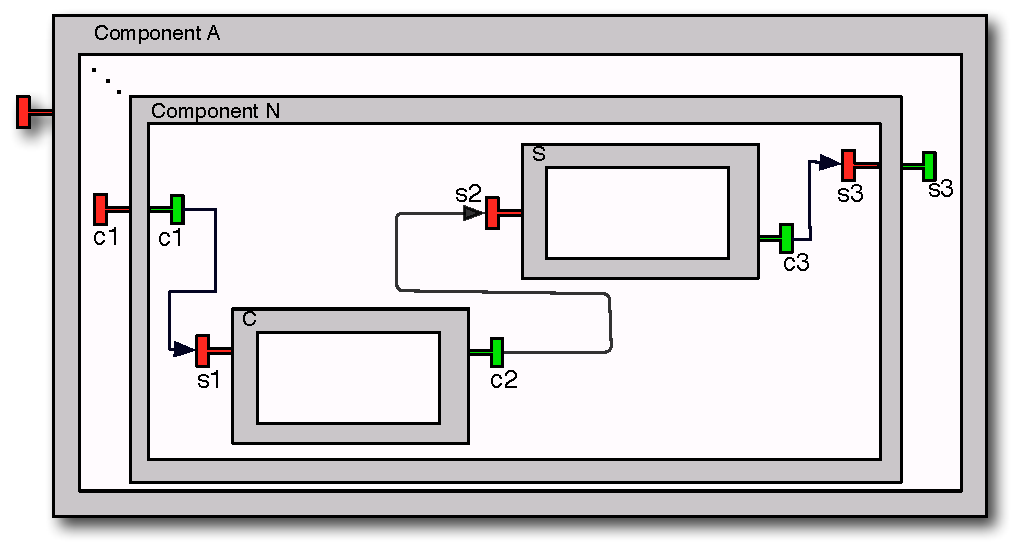
\includegraphics[scale=0.7]{figures/chapter4/bindings.pdf}
		\caption{\textsf{binding} examples}
		\label{fig:bindingsdemo}		
	\end{figure}		

	\noindent From left to right, the three bindings illustrated by Figure \ref{fig:bindingsdemo} are depicted by
	Listing \ref{lst:exbindings}.

	\lstinputlisting[language=Coq, stepnumber=1, 
	                        caption={\textsf{binding} examples in \textsc{Mefresa}}, 
	                        label=lst:exbindings]{listings/chapter4/bindings.tex}

	\noindent where \textbf{pb} is \textsf{(Ident "Component A" :: ... :: Ident "Component N" :: nil)}, i.e., the adequate 
	\textsf{path} for the bindings hold by the \textsf{component} named \textit{"Component N"}.


	%maybe i should some more prose and a complete component term ==> component term needed to justify language
	
\subsubsection{A complete example}
		
				
		Having discussed the three core elements of the \ac{GCM}, it still remains to see them all together at once.
	For the sake of clarity, in the following we show how the aforementioned
	\textsf{component} \textit{"Component N"} is represented in \textsc{Mefresa}. First, let us
	 mechanize its subcomponent \textit{"C"}. Listing \ref{lst:rex1} depicts such a task.
		
	\lstinputlisting[language=Coq, stepnumber=1, 
	                       caption={Model for \textsf{component} \textit{"Component N"} (part 1 of 3)}, 
	                       label=lst:rex1]{listings/chapter4/rex1of3.tex}
	
	
	\noindent Lines 1-4 define some parameters for this example. Parameter \textbf{p}
	stands for the \textsf{path} of \textsf{component} \textit{"Component N"}. Then,
	 \textsf{iclC}, \textsf{sigS1} and \textsf{sigC2} stand for the implemenetation class
	 of \textsf{component} \textit{"C"}, \textsf{signature} of \textsf{interface S1} and 
	 \textsf{signature} of \textsf{interface C2}, respectively. Line 6 defines
	 the \textsf{path} for \textsf{component} \textit{"C"} by appending the appropriate \textsf{identifier}.
	 The definition of \textsf{component} \textit{"C"} \textit{per se} starts at line 8. Its understanding
	 should pose no doubt. It is set with the default control level value \textsf{Configuration},
	 has no subcomponents --- thus represented by an empty list (line 11) --- 
	 features two interfaces adequately
	 defined in lines 13-16, and has no bindings (line 18).
	
	
	\lstinputlisting[language=Coq, stepnumber=1, 
	                      caption={Model for \textsf{component} \textit{"Component N"} (part 2 of 3)}, 
	                       firstnumber=19,
	                      label=lst:rex2]{listings/chapter4/rex2of3.tex}	
	
	
	\noindent	 Sub\textsf{component} \textit{"S"} has the same structure and 	
	is naturally defined analogously. Its mechanization is depicted by Listing \ref{lst:rex2}.
	Note that both \textsf{component}s \textit{"S"} and \textit{"C"} possess the same 
	\textsf{path} (line 23), we assign a new variable for the sake of clarity.
	 
	\lstinputlisting[language=Coq, stepnumber=1, 
	                      caption={Model for \textsf{component} \textit{"Component N"} (part 3 of 3)}, 
	                       firstnumber=36,
	                      label=lst:rex3]{listings/chapter4/rex3of3.tex}		
	
	\noindent For last, composite \textsf{component} \textit{"Component N"} is illustrated by
	Listing \ref{lst:rex3}. The careful reader may notice the definition of the variable \textsf{pN}
	(line 39). This, is subsequently used as \textsf{path} for \textsf{component} \textit{"Component N"}'s
	\textsf{interface}s and \textsf{binding}s. Indeed, all of its constituents (sub\textsf{component}s,
	\textsf{interface}s and \textsf{binding}s) possess the same \textsf{path}. 
	
		The remaining of its mechanization should pose no doubt. It mainly differs from
	the two precedent mechanizations (Listing \ref{lst:rex1} and Listing \ref{lst:rex2}) in
	that it also possesses sub\textsf{components}, \textsf{interface}s of \textsf{internal} visibility,
	and \textsf{binding}s.
	

\subsection{Well-formed component architectures}
\label{sub:wellformed}

	 The above definition of the \ac{GCM} core elements allowed us to see how to compose components.
	 Indeed, by exploiting their hierarchical structure one can build arbitrary complex
	 architectures. Yet, randomly constructing these by solely respecting the 
	 inherent typing rules for the \textsf{component}, \textsf{interface}
	 and \textsf{binding} structures, is naturally insufficient w.r.t.
	 the \ac{GCM} specification compliance. In order to be certain that we are
	 building valid \ac{GCM} architectures we need to formalize its requirements.
	
%%%%
	
		Let us define a predicate concerning the \textit{well-formedness} of a \textsf{component}.
	Listing \ref{lst:wfcomp} depicts such predicate. %, where the notation \textsf{(object-->field)} is used 
	%for projections: \textsf{(c-->subcomps)} stands for the subcomponents of \textsf{c}, etc.			
	
	
		\lstinputlisting[language=Coq, stepnumber=1, 
	                        caption={well-formed \textsf{component} definition}, 
	                        label=lst:wfcomp]{listings/chapter4/wfcomp.tex}

	\noindent Basically, a \textsf{component} is \textit{well-formed} if all its subcomponents
	are individually well-formed (line 3), and do not possess common identifiers (line 4). Further,
	its interfaces and bindings must also be well-formed (lines 5-6). 

	
	The intended meaning of the
	\textsf{unique\_ids} predicate should be clear from its name. 
	Listing \ref{lst:uniqueids} depicts its definition.
	
	\lstinputlisting[language=Coq, stepnumber=1, 
	                        caption={\textsf{unique\_ids} predicate definition}, 
	                        label=lst:uniqueids]{listings/chapter4/uniqueids.tex}

	\noindent It is composed by two constructors: \textsf{Unique\_Base} and \textsf{Unique\_Step}.
	The former simply states that an empty list has indeed unique identifiers. The latter covers
	the case when the parameter \textsf{l} is composed by a head element
	\textsf{c} and a tail list \textsf{r} (line 13). The subsequent two premisses
	ensure that \textsf{c}'s identifier is not equal to the \textsf{component}s' identifier 
	in the tail \textsf{r} (line 14), and for last, the predicate itself is applied to the tail
	\textsf{r} (line 15). Concerning the \textsf{not\_in\_l} predicate, it is essentially	
	defined in the same manner. The \textsl{NotInNil} constructor deals with the case
	when the parameter \textsf{l} is empty (lines 2-3). The \textsf{NotInStep} constructor deals with the
	more interesting case, when \textsf{l} is composed by a head element \textsf{c} 
	and a tail \textsf{r} (line 5).	\textsf{c}'s identifier is checked against
	parameter \textsf{i} (line 6), and the predicate itself is recursively applied
	to the tail \textsf{r} (line 7).
	
	
		Regarding \textsf{component}'s \textsf{interface}s, the sole requirement is that they are uniquely identifiable
	by their \textsf{id} and \textsf{visibility} values. Listing \ref{lst:unique} formalizes
	this constraint.			
	
	\lstinputlisting[language=Coq, stepnumber=1, 
	                        caption={\textsf{well\_formed\_interfaces} predicate definition}, 
	                        label=lst:unique]{listings/chapter4/unique.tex}
	
	\noindent Indeed, the \textsf{not\_in\_l\_pairs} predicate does the main work.
	The expression \textsf{not\_in\_l\_pairs i v l} should be read as: there is no
	\textsf{interface} in \textbf{l} that possesses both the same identifier and
	visibility values as \textbf{i} and \textbf{v}, respectively.	
	The constructor \textsf{NotInPairsNil} covers the case where \textbf{l}
	is empty --- it is simply true by definition (line 2). 
	The constructor \textsf{NotInPairStep} accounts for the case where \textbf{l}
	contains at least one element: a head element \textbf{int} 
	followed by a tail \textbf{r} (line 4). 	
	The arguments \textbf{i} and \textbf{v} are checked against the identifier and
	\textsf{visibility} values of \textbf{int} (line 5), and finally the same process is applied to
	the tail \textbf{r}, making the predicate recur (line 6).
	
		The understanding of the \textsf{unique\_pairs} predicate should pose no doubt, it
	essentially follows the same rationale, and relies on \textsf{not\_in\_l\_pairs} to achieve
	its intended significance.


		Before further proceeding into well-formedness concerns, let us define an auxiliary function
	concerning the indexation of \textsf{interface}s. Listing \ref{lst:itfindex} defines a function
	retrieving one \textsf{interface} from a list of \textsf{interface}s by its identifier and
	\textsf{visibility} values.

\lstinputlisting[language=Coq, stepnumber=1, 
	                        caption=Function to find an \textsf{interface} by its identifier and \textsf{visibility} values, 
	                        label=lst:itfindex]{listings/chapter4/itfindex.tex}

	\noindent Its comprehension is straightforward. The \textit{head} element \textsf{i}
	of parameter \textsf{l} is checked for its identifier and \textsf{visibility} values (line 5). 
	Should they be equal to parameters \textsf{id} and \textsf{v}, respectively, 
   \textsf{interface} \textsf{i} is returned (line 6). Otherwise,
   the function recurs in the \textit{tail} \textsf{r} (line 8). Naturally, no \textsf{interface} is returned if 
   \textsf{l} is empty (line 4). Moreover, a convenient notation is defined (line 11): \textsf{l[id, v]} stands
   for \textsf{get\_interface id v l}.
   
    

%%%binding wf
	The last remaining piece concerns the well-formedness of \textsf{binding}s. 
	Listing \ref{lst:wfbinding} illustrates its definition.

			\lstinputlisting[language=Coq, stepnumber=1, 
	                        caption={\textsf{well\_formed\_bindings} predicate definition}, 
	                        label=lst:wfbinding]{listings/chapter4/wfbinding.tex}
	
	\noindent The careful reader may notice one particularity regarding the definition of the
	\textsf{well\_formed\_bindings} predicate: unlike  \textsf{well\_formed\_component} and
	\textsf{well\_formed\_interfaces}, it takes more than one parameter into account.
	A binding is hold by a component and serves as a means for 
	components to communicate with each other, and thus cannot 
	exist by itself. As such, it should come as no surprise that its
	well-formedness depends on its surroundings, i.e. the
	components and interfaces involved in its definition.
			
	Regarding the	mechanization depicted by Listing \ref{lst:wfbinding}, its 
	understanding should pose no doubt.  Basically, the predicate \textsf{valid\_binding}
	is applied to all bindings $b \in lb$ (line 9). This, performs a case analysis
	on \textit{b} and its validity is checked depending on whether it is a 
	\textsf{normal}, \textsf{export} or \textsf{import binding} (lines 2-5).
	 For instance, Listing \ref{lst:nmbinding} depicts the \textsf{normal\_binding} predicate.
		
	\lstinputlisting[language=Coq, stepnumber=1, 
	                        caption={\textsf{normal\_binding} predicate definition}, 
	                        label=lst:nmbinding]{listings/chapter4/normalbinding.tex}
	
	\noindent  A \textsf{normal binding} establishes a binding between two sub\textsf{component}s, and	
	is composed by four identifiers denoting
	(1) the name of the \textsf{component} holding the \textsf{client interface}, (2) the name
	of this \textsf{client interface}, (3) the name of the \textsf{component} holding the \textsf{server interface}, and
	finally (4) the name of this \textsf{server interface}. Therefore, checking its validity boils down
	to ensuring that these identifiers refer to existing client and server interfaces.
	The parameters \textsf{idC1} and \textsf{idC2} contain the name of the \textsf{component}s
	involved in the \textsf{binding}. These are both supposed to be indexed in \textsf{lc} (line 3),
	if that is not the case it means that the binding is not valid and \textsf{False} is 
	returned (line 9). If both components \textsf{c1} and \textsf{c2} are found, then 
	\textsf{idI1} and \textsf{idI2} are supposed to be indexed in their list of \textsf{interface}s, respectively.
	Further, since it is a \textsf{normal binding}, it implies that it is established between 
	two \textsf{external} interfaces (line 5). Failure to find the referred \textsf{interface}s means that
	the binding is not valid and \textsf{False} is returned (line 7). Otherwise,
	its validity depends on whether 
	the \textsf{interface}s \textsf{i} and \textsf{i'} are indeed of \textsf{client} and \textsf{server} roles, respectively (line 6).
			
		As expected, the predicates \textsf{export\_binding} and \textsf{import\_binding} are defined
	analogously. The main difference lies in the fact that these \textsf{binding}s are not between two sub\textsf{component}s,
	but between a parent \textsf{componen}t and one sub\textsf{component} (or vice-versa). 
	

\subsubsection{A first well-formedness proof}
	
	%running example
	Having defined	 our well-formedness predicates it is time to see them in action. Let us retake our
	running example concerning \textsf{component} \textit{"Component N"} discussed in
	Subsection \ref{sub:core} (see Listing \ref{lst:rex1}, Listing \ref{lst:rex2} and Listing \ref{lst:rex3}). 
	
		First, let us reason about its sub\textsf{component}s well-formedness. Lemma \ref{th:wflemmaexC}
	addresses the well-formedness of \textsf{component} \textit{"C"}.
				
			
	\begin{lemma} \label{th:wflemmaexC} 
	\lstinputlisting[language=Coq, numbers=none]{listings/chapter4/wflemmaC.tex}				
	
		We start by applying the \textsf{WellFormedComponent} constructor, which yields
		four subgoals to discharge.			
		  The first and second subgoals concern its subcomponents: their 
		individual well-formedness and the uniqueness of their identifiers.		
		Since it has no	subcomponents both premisses are trivially established. 
			
			The third subgoal regards the well-formedness of its interfaces. These need
			to be uniquely identifiable by the tuple composed by their identifier and
			visibility values. It is clearly the case as it only possesses two external interfaces
			named \textsf{s1} and \textsf{c2}.			
			
			Finally, the fourth subgoal requires the well-formedness of its bindings. This is also
			trivially proved as it is a primitive component and thus has no bindings.
			And therefore the proof concludes. \qed
	\end{lemma}				

			
	\noindent As expected, proving the well-formedness of \textsf{component} \textit{"S"} follows
	the same rationale. Indeed, both	possess the same structure. Regarding 
	\textsf{component} \textit{"Component N"}, its well-formedness is tackled by Lemma \ref{th:wflemmaexN}. 
				
	\begin{lemma} \label{th:wflemmaexN} 
	\lstinputlisting[language=Coq, numbers=none]{listings/chapter4/wflemmaN.tex}				
	
		Applying \textsf{WellFormedComponent} yields four subgoals to prove.	
		
		It possesses two subcomponents (\textsf{component} \textit{"C"} 
		and \textsf{component} \textit{"S"}), both are well-formed as previously discussed.	Further,
		their identifiers are different, and therefore the first two subgoals are easily discharged.
		
			It features four interfaces. Two of external visibility, and two of internal visibility.
		Indeed,	 some share the same identifier, yet, these are of different visibility value, and thus still
		uniquely identifiable.
		
			For last, its three bindings are established from and to existent components/interfaces, and from
			client to server. Thus, also well-formed, and the proof concludes. 	\qed
	\end{lemma}	
	

%\subsubsection{General properties: well-formedness corollaries}	
	
	
\subsection{Well-typed component architectures}
\label{sub:welltyped}

	A \textsf{component} may be well-formed but still unable to start execution. Indeed, its
	 well-formedness guarantees involve important aspects regarding its composition, yet,
	 further insurances are needed for the overall good functioning of the system in terms of its 
	 application dependencies. These are dictated by simple typing rules (see \cite[p. 22]{ETSI2009:GCMADL}).	 
	 
		An \textsf{interface} possesses \textsf{cardinality} and \textsf{contingency} attributes. These determine
	its supported communication model and the guarantee of its functionality availability, respectively.
	For instance, as dictated by the \ac{GCM} specification, for proper system execution 
	we must ensure that \textsf{singleton} \textsf{client} \textsf{interface}s 
	are bound at most once. Indeed, for \textsf{client} \textsf{interface}s only those with \textsf{multicast} \textsf{cardinality}
	are allowed to be bound more than once. 
	
		Analogously, similar constrains apply to the \textsf{interface}s' \textsf{contingency} attribute. An \textsf{interface} 
	of \textsf{mandatory}	\textsf{contingency}  is guaranteed to be available at runtime. This is rather obvious for \textsf{server}
	\textsf{interface}s as they implement one or more service methods, i.e., they do have a functionality of their own. \textsf{Client}
	\textsf{interface}s however, are used by service methods that require other service methods to perform their task. It therefore follows
	that a \textsf{client} and \textsf{mandatory} \textsf{interface} must be bound to another \textsf{mandatory} \textsf{interface} of
	\textsf{server} \textsf{role}.  As expected, \textsf{interface}s of \textsf{optional} \textsf{contingency} are not guaranteed to be available.
			
	\textsc{Mefresa} captures these requirements by defining a well-typed predicate as depicted by Listing \ref{lst:wtyped}.


	\lstinputlisting[language=Coq, stepnumber=1, 
	                        caption={\textsf{well\_typed} predicate definition}, 
	                        label=lst:wtyped]{listings/chapter4/wtyped.tex}

	\noindent  Its definition is straightforward, it is a simple conjunction between two more interesting 
	predicates: \textsf{sound\_cardinality} and \textsf{sound\_contingency}. Listing \ref{lst:scont} depicts the latter.
	
		
	\lstinputlisting[language=Coq, stepnumber=1, 
	                        caption={\textsf{sound\_contingency} predicate definition}, 
	                        label=lst:scont]{listings/chapter4/scont.tex}
	
  \noindent As shown by the \textsf{sound\_contigency} predicate we split its definition
		into \textsf{subc\_client\_external\_mandatory\_itfs\_are\_bound} 
       and \textsf{client\_internal\_mandatory\_itfs\_are\_bound}. Indeed,	the former checks the \textsf{external}
       \textsf{interfaces}, while the latter the \textsf{internal} ones. 
           
       
	       \lstinputlisting[language=Coq, stepnumber=1, 
	                        caption={\textsf{client\_internal\_mandatory\_itfs\_are\_bound} predicate definition}, 
	                        label=lst:cimi]{listings/chapter4/cimi.tex}
       
      Listing \ref{lst:cimi} depicts the \textsf{client\_internal\_mandatory\_itfs\_are\_bound} predicate.      
      Basically, we need to check that for all \textsf{client}, \textsf{internal}, and
       \textsf{mandatory} \textsf{interfaces} of some \textsf{component} \textbf{c} (lines 3-4), 
       their \textsf{interface} recipients list originating from \textsf{export bindings} 
       are non-empty --- i.e. at least bound once --- (lines 5-7) and of \textsf{mandatory} \textsf{contingency} (line 8). 	
	   Naturally, the same applies recursively to the remaining of the \textsf{component} hierarchy (lines 9-10).	
	
		  As expected, the \textsf{subc\_client\_external\_mandatory\_itfs\_are\_bound}  predicate is defined analogously
	  w.r.t. the sub\textsf{component}s \textsf{external} \textsf{interface}s. For the sake of completeness,
	  Listing \ref{lst:cemi} depicts its definition.
	  
	   \lstinputlisting[language=Coq, stepnumber=1, 
	                        caption={\textsf{subc\_client\_external\_mandatory\_itfs\_are\_bound} predicate definition}, 
	                        label=lst:cemi]{listings/chapter4/cemi.tex}
	
	%%%should i add text here?
		
%%%%%%	
\subsubsection{A first well-typedness proof}
	
	Retuning to our running example from Subsection \ref{sub:core}, let us discuss
	\textsf{component} \textit{"Component N"}'s well-typedness.
	
	 First, we need to establish that \textsf{component} \textit{"Component N"} has indeed
	 a sound \textsf{contingency}. Lemma \ref{th:scontlemma} addresses this concern.
	 	 
		
\begin{lemma} \label{th:scontlemma} 
	\lstinputlisting[language=Coq, numbers=none]{listings/chapter4/scontlemma.tex}		
	
	By unfolding the statement to prove, we can see that it is actually a 
	conjunction of two predicates: subc\_client\_external\_mandatory\_itfs\_are\_bound 
	and client\_internal\_mandatory\_itfs\_are\_bound. 
	
		 For the former we start by applying its constructor \textsf{CEMI\_Bound} and
	get two subgoals to discharge. The first one requires that all subcomponents'
	client, external and mandatory interfaces are indeed bound, 
	while the second one recursively requires the same for the component hierarchy 
	inner levels. 
		Component "Component N" contains two subcomponents: "C" and "S". Both
	possess one client interface, "c2" and "c3", respectively. Yet, only "c2" is of mandatory 
	contingency, and it is indeed adequately bound through a normal binding
	to "s2" (which is also of mandatory contingency). Proving the second subgoal 
	is straightforward: both subcomponents "C" and "S" are primitive, thus possess no 
	subcomponents. And therefore subc\_client\_external\_mandatory\_itfs\_are\_bound 
	is discharged.
	
		Proving client\_internal\_mandatory\_itfs\_are\_bound follows the same rationale.
	Only the interface "c1" from component "Component N" is concerned and it is indeed
	adequately bound to "s1". \qed
\end{lemma}

	\noindent The demonstration that \textsf{component} \textit{"Component N"}
	has a sound cardinality follows the same spirit. Basically, 	we need to exhaustively
	check that all concerned \textsf{interface}s are meeting the cardinality-related 
	requirements. For such simple \textsf{component} architecture, it is easy to see
	that it is indeed the case as all the present \textsf{interface}s are of \textsf{singleton}
	\textsf{cardinality} and are all bound at most once. 
	
		Finally, we can show that \textsf{component} \textit{"Component N"} is 
	indeed well-typed. This is illustrated by Lemma \ref{th:wtlemma}.
		

\begin{lemma} \label{th:wtlemma} 
	\lstinputlisting[language=Coq, numbers=none]{listings/chapter4/wtlemma.tex}		
		Establishing the well-typedness of component "Component N" boils down to
	proving that it has a sound contingency and a sound cardinality. This is clearly the case
	as previously discussed. \qed
\end{lemma}

	%%should i put text here..

%%%%
\subsection{Well-formedness and well-typedness decidability}
\label{sub:wfdec}


	A \textsf{component} that is both well-formed and well-typed is said to be ready to 
	start execution. The definition of these predicates gives us the ability to interactively prove inside Coq	
	that a \textsf{component} system can, or not, start its execution. The burden of such a demonstration for one  
	component \textsf{c} will therefore inherently depend on the complexity of \textbf{c}. In fact, one may wonder
	about the feasibility of undertaking such proof, i.e., whether it is indeed possible to actually prove
	or disprove that \textbf{c} is well formed and well typed\footnote{It should be noted that
	we are in the context of Coq's constructive logic, theorems that are true in 
	classical logic (i.e. the excluded middle) may not be provable in Coq.}.	 In other words, it is
	worth knowing that both predicates are \textit{decidable}.
	
		First, we need a predicate expressing decidability. Listing \ref{lst:dec} depicts one such
	predicate.		
	
	   \lstinputlisting[language=Coq,  
	                        caption=\textsf{decidable} predicate definition, 
	                        label=lst:dec]{listings/chapter4/dec.tex}
	
	\noindent Its definition is rather simple: it takes one proposition and returns the disjunction of this 
	proposition itself with its negation. For our purposes, we shall use it for our
	well-formedness and well-typedness predicates. Indeed, proving them decidable is of 
	paramount importance, it ensures the existence of an algorithm capable of automatically 
	determining their valuation.

	Generally, there are two approaches for proving a predicate's decidability. On the one hand,
	one can attempt to prove it by exploiting the structure of the involved parameters, showing that for all
	of its constructors it is indeed possible to infer a \textit{True} or \textit{False} valuation. 
	On the other hand, one can	write a function that acts as its computational counterpart, i.e.,
	it returns a boolean value, \textit{true} or \textit{false}, in accordance with the predicate's 
	valuation. Then, one needs to show that this function is \textit{sound} --- whenever it returns 
	\textit{true} the predicate's valuation is \textit{True} ---, and \textit{complete} --- whenever
	 the predicate's valuation is \textit{True}, the function returns \textit{true}. Such 
	 functions are often called \textit{decision procedures}. Finally, proving the predicate's decidability
	 has now become trivial since it is intrinsically related with this boolean function.
	
		In the following, we use the first approach for demonstrating the decidability of the
	\textsf{well\_formed\_component} predicate, and the second approach for tackling the decidability 
	of the \textsf{well\_typed} predicate. As we shall see in detail in Chapter \ref{chap:extraction},
	this choice is related with software engineering aspects: we need the functional code
	computing the well-typedness of a \textsf{component}, while an analogous
	function for the well-formedness would be redundant.
	

\subsubsection{Well-formedness decidability}
	
				
		As shown by Listing \ref{lst:wfcomp}, the \textsf{well\_formed\_component} predicate is
	composed by other predicates: \textsf{unique\_ids}, \textsf{well\_formed\_interfaces}, and
	\textsf{well\_formed\_bindings}. Naturally, proving their decidability is required in order
	to demonstrate that  \textsf{well\_formed\_component} is decidable.	
	
		For instance, let us consider the \textsf{unique\_ids} predicate. As shown by Listing
		\ref{lst:uniqueids}, its definition includes the \textsf{not\_in\_l} predicate (see Listing \ref{lst:uniqueids}). As such,
		the first step is to prove its decidability. This is demonstrated by Lemma \ref{th:notindec}. 
				
		\begin{lemma} \label{th:notindec} 
		\lstinputlisting[language=Coq, numbers=none]{listings/chapter4/notindec.tex}		
		
			We start by applying induction on the structure of \textsf{l}, and thus
		obtain two subgoals. Both require the original goal but applied 		
		to an empty list, and to a list composed by a head element \textsf{c}
		and a tail \textsf{l}.
		
			The first subgoal is trivial. We recall that the \textsf{decidable} predicate 
		actually stands for a disjunction. In particular, for this 
		case: \textsf{not\_in\_l id nil $\lor$ $\neg$not\_in\_l id nil}. Its left-hand side
		proposition its evidently true. Proving \textsf{not\_in\_l id nil} can easily be achieved by applying
		the \textsf{NotInNil} constructor, at which point we only need to show that
		\textsf{nil = nil}, which is discharged by reflexivity. 
		
			The second subgoal requires the demonstration of \textsf{decidable (not\_in\_l id (c::l))} by assuming
		\textsf{decidable (not\_in\_l id l)} as induction hypothesis. At this point we can safely assume that
		\textsf{(c ->id) = id} is either true or false. 
		
		For the first case, we can show that the right-hand side
		of our goal is true. Indeed, since \textsf{(c ->id)} is equal to \textsf{id}, then it is easy to see that
		\textsf{not\_in\_l id (c::l)} is false. Thus, we need to prove the negation of false, which is a		
		tautology. 
		
		For the second case, we need to use the induction hypothesis. We  know that 
		\textsf{(not\_in\_l id l)} is either true or false. If it this true, then we can show that
		\textsf{not\_in\_l id (c::l)} is also true. Indeed, since \textsf{(c ->id) = id} is false
		we have all the ingredients to discharge this subgoal by applying the \textsf{NotInStep} 
		constructor. If it is false, then it follows that \textsf{not\_in\_l id (c::l)} is also false, as we
		have in context the negation of one of its premises. And thus the proof concludes. \qed		
		\end{lemma}
				
		Having demonstrated \textsf{not\_in\_l}'s decidability, we are now in a position to
	address the \textsf{unique\_ids} predicate. Its decidability is discussed
	by Lemma \ref{th:uniquedec}.	
	
	\begin{lemma} \label{th:uniquedec} 
		\lstinputlisting[language=Coq, numbers=none]{listings/chapter4/uniquedec.tex}		
		
				We start by applying induction on the structure of \textsf{lc}. This, naturally yields
			two subgoals: we now need to demonstrate the original goal for an empty list,
			and then for a list composed by a head element \textsf{c} and a tail list \textsf{l}.
			
				The first subgoal is trivial, we can easily demonstrate \textsf{unique\_ids nil}
			by applying its \textsf{Unique\_Base} constructor.				
				
				The second subgoal is more elaborated. From the induction hypothesis
			we know that \textsf{unique\_ids lc} is either true or false. Further, 
			from Lemma \ref{th:notindec} we know that this is also the case for 
			\textsf{not\_in\_l (c ->id) lc}. We need to consider all their pairwise 
			combinations, and thus we have four cases to deal with. 
			
				For the first case, we have both assumptions with a valuation of true. 
				It this therefore easy to show that \textsf{unique\_ids (c :: lc)} holds by applying
			the \textsf{Unique\_Step} constructor.
			
				The remaining three cases possess at least one assumption with
			a valuation of false. Thus, it is always possible to show that
			\textsf{$\neg$ unique\_ids (c :: lc)} holds, as we always have
			the negation of one of its premises in context. And thus we can conclude
			the proof. \qed
	\end{lemma}
	
		\noindent Proving the decidability of the \textsf{well\_formed\_interfaces} and
	\textsf{well\_formed\_bindings} predicates follow the same rationale. We account for
	all possible cases by recurring to structural induction, and reasoning symbolically on
	the parameters. However, it should be noted that \textsf{well\_formed\_component c} 
	also possesses a premise involving a nested recursive call: \textsf{$\forall c',\ c' \in (c.subcomps)
	\rightarrow well\_formed\_component \ c'$}. Alas, coping with 
	such definitions in Coq is somewhat cumbersome, and requires delving into its
	intricacies. In the following, we demonstrate an approach that can be seen as a general
	recipe for dealing with such cases.
	
			First, let us prove an auxiliary lemma that is somewhat peculiar: it is possible to decide that
	all components in an empty list are well-formed. Lemma \ref{th:wflnil} demonstrates this.			
			
		\begin{lemma} \label{th:wflnil} 
		\lstinputlisting[language=Coq, numbers=none]{listings/chapter4/wflnil.tex}
		
		We can easily show the left-hand side of our goal: 
		$\forall c,\ c \in nil \rightarrow$ well\_formed\_component\ c. This means that
		we have $c \in nil$ as an assumption, which is always false.				
		Since from false anything follows, we can conclude the proof. \qed
	\end{lemma}				


	\noindent Having dealt with the case where the list of \textsf{component}s is empty,
	let us now cope with  the case where it is composed by a head element and a tail.
	For this case however, as demonstrated by Lemma \ref{th:wfcons}, we shall use
	some parameters to establish the proof. Basically, the parameters include the
	decidability of the well-formedness of a \textsf{component} \textbf{c}, and the 
	decidability of the well-formedness of all \textsf{component}s in a list \textbf{lc}.
	Then, we want to show that all \textsf{component}s in (\textsf{cons} \textbf{e} \textbf{lc})
	are also well-formed. 

		\begin{lemma} \label{th:wfcons} 
		\lstinputlisting[language=Coq, numbers=none]{listings/chapter4/wfcons.tex}		
			
			From the \textsf{Hc} hypothesis we know that well\_formed\_component \textbf{c}
			is either true or false. If it is false, then it evidently follows that $\neg (\forall e,\
			e \in (cons\ c\ lc) \rightarrow$ well\_formed\_component e). We only need to
			instantiate \textbf{e} with \textbf{c} to see that it is the case. If it is true however,
			we need to account for two other possibilities: from \textsf{Hlc} we know that ($\forall$ e, 
			e $\in$ lc $\rightarrow$ well\_formed\_component e) is either true or false.
			If it is true, then we have all the necessary assumptions to prove that
			the left-hand side of our goal holds:
			if \textbf{e} is instantiated with \textbf{c}, then we can show it with
			\textsf{Hc}, otherwise if $\textbf{e} \in \textsf{lc}$, then we can show it
			with \textsf{Hlc}. If it is false however, then we can show the right-hand side
			of our goal by analogous reasoning. \qed
	\end{lemma}	
	
		 The last remaining ingredient before proceeding to the main proof is
	depicted by Lemma \ref{th:wfclc}. Basically, we prove the decidability of the well-formedness of 
	all \textsf{component}s member of a list, while having as parameter the 
	decidability of the well-formedness of all \textsf{component}s. Indeed, 
	it seems a rather strange lemma to prove. However, it is of paramount 
	importance for the applicability of this approach. 
	We exhibit its proof with the associated Coq script in order
	to further emphasize the peculiarity of the approach. 
					
	\begin{lemma} \label{th:wfclc} \textit{well_formed_component_lc_dec:}
		\vspace{-0.2cm}
		\lstinputlisting[language=Coqfix, numbers=left, numberfirstline=false, stepnumber=1, firstnumber=2]{listings/chapter4/wfclc.tex} 
		
		%\vspace{-0.8cm} \qed
	\end{lemma}	
	
	\noindent  The first thing to note is the use of the \textsf{fix} construct (line 5). This allows
	to define anonymous recursive functions. Basically, the proof is achieved by defining
	a recursive function that pattern matches on its parameter \textsf{lc} and uses Lemma \ref{th:wflnil}
	and Lemma \ref{th:wfcons} to adequately cover all the cases (lines 8-10). For last, the careful reader may 
	wonder about the use of \textit{Defined} instead of \textit{Qed} (line 12). 
	This makes Coq keep the proof of Lemma \ref{th:wfclc} --- it exposes its 
	recursive nature to a caller --- while with \textit{Qed} it would become 
	\textit{opaque}. 
		
		Finally, we are in a position to prove the decidability of the \textsf{well\_formed\_component}	
	predicate for all \textsf{component}s \textbf{c} as demonstrated by Theorem \ref{th:wfdec}. 
	We also exhibit its proof as a Coq script 
	to illustrate how the approach described so far is put into practice.	
	
	\begin{theorem} \label{th:wfdec} \textit{well_formed_component_dec:}
	\vspace{-0.2cm}
		\lstinputlisting[language=Coq, numbers=left, firstnumber=2]{listings/chapter4/wfdec.tex}	
		%\vspace{-0.9cm} \qed
	\end{theorem}

	\noindent We start the proof by performing structural induction on the first argument through
	the \textsf{fix} tactic\footnote{Not to be confused with the previously mentioned 
	\textsf{fix} construct for recursive functions.} and introduce in the 
	context \textsf{component} \textbf{c}'s constituents (identifier, path, implementation class, ...) (line 4). 
	The \textsf{fix} tactic also introduces a new hypothesis in the context, 
	named as the current theorem, and with the same type as the goal. Indeed, this is an odd
	behaviour, and one may be tempted to use this new hypothesis to discharge the goal, but that would make
	Coq reject the proof. In short, proofs done with \textsf{fix} are required to satisfy a syntactic 
	\textit{guardedness} criterion, and attempting to directly discharge a goal with the hypothesis it
	introduces violates this criterion.	
	
		We introduce the proof that all sub\textsf{component}s of \textbf{c} are
	well-formed into our context and name it \textsf{IHp\_dec} (lines 5-6). Further, we
	remove the hypothesis introduced by \textsf{fix} since we will not use it anymore (line 7).
	Then, we use the \textsf{Guarded} command to check that Coq's guardedness 
	condition is satisfied (line 8). It is not a tactic, it does not affect the state of the
	proof. Its sole purpose is to inform about the compliance of this guardedness condition
	at the current state of the proof, rather than having to wait until its conclusion.

		At this point, the main work for this proof is done. The remaining simply
	accounts for all possible cases regarding the well-formedness decidability of 
	the involved predicates (lines 10-12), and discharges them adequately (lines 16-17).
	

		Finally the decidability of our \textsf{well\_formed\_component} is proved. Undeniably, 
	the burden of this approach is considerable. This is mainly due to the way Coq is able to cope
	with nested definitions such as the \textsf{component} datatype. Moreover, the behaviour 
	of the \textsf{fix} tactic is rather undocumented, and is generally not recommended. In fact, even in
	\textit{Cocorico}\footnote{Cocorico is the official Coq wiki, also known as \textit{The nonterminating Coq wiki}: \url{http://coq.inria.fr/cocorico/Home}} it is stated that \textit{"it is not advisable to use it (unless you know what you do)"}.
	Alas, there are situations where it is indeed required. Nevertheless, for more details on its intricacies the reader is pointed to 
	Gim\'enez's tutorial on recursive types \cite{Giménez98atutorial} for a very brief discussion on its use. 
	
	
	
\subsubsection{Well-typedness decidability}


	Having demonstrated the \textsf{well\_formed\_component} predicate decidable, it is time to cope
	with the \textsf{well\_typed} predicate. As mentioned earlier, we shall use a different approach
	to tackle this task: we define some functional code that act as the computational counterpart of the \textsf{well\_typed}
	predicate.
		
			Basically, we need a function that returns the boolean value \textit{true} whenever
		a \textsf{component} is well-typed, and the boolean value \textit{false} otherwise. Further, it must be able
		to do it for all \textsf{component}s given as input. Listing \ref{lst:wtbool} depicts such function.

		
	\lstinputlisting[language=Coq,  
	                        caption=\textsf{well\_typed\_bool} function definition, 
	                        label=lst:wtbool]{listings/chapter4/wtbool.tex}		
	
			
	\noindent Basically, it follows the same spirit as the \textsf{well\_typed} predicate (see Listing \ref{lst:wtyped}),
	except that it is composed by boolean functions rather than predicates. With no surprise, the definition
	of the \textsf{sound\_contingency\_bool} function also follows the same spirit as the \textsf{sound\_contingency}
	predicate (see Listing \ref{lst:scont}). Listing \ref{lst:soundcontbool} depicts its definition.	
	
		\lstinputlisting[language=Coq,  
	                        caption=\textsf{sound\_contingency\_bool} function definition, 
	                        label=lst:soundcontbool]{listings/chapter4/soundcontbool.tex}
	
	
	\noindent Indeed, the actual work is carried by the two boolean functions
	\textsf{client\_internal\_mandatory\_itfs\_are\_bound\_bool} and 
	\textsf{subcomponents\_client\_external\_mandatory\_itfs\_are\_bound\_bool}
	--- the computational counterparts of the predicates depicted in Listing \ref{lst:cimi} 
	and Listing \ref{lst:cemi}, respectively. Listing \ref{lst:cimitfs} depicts the former.		


	\lstinputlisting[language=Coqfix,  
	                        caption=\textsf{client\_internal\_mandatory\_itfs\_are\_bound\_bool} function definition, 
	                        label=lst:cimitfs]{listings/chapter4/cltintmandbool.tex}


   \noindent %Indeed, the definition of this nested recursive function is all but natural.
   %This is related with Coq's termination checker. We need to write it in this way so that Coq can automatically
   %infer that it terminates. 
 % Nevertheless, 
   Its understanding should pose no doubt. Basically, it uses an auxiliary function
   \textsf{client\_internal\_mandatory\_itfs\_are\_bound\_bool\_one} to check the \textsf{interface}s at the current 
   hierarchical level (line 4) and then recurs on the inner levels, i.e., on the 
   sub\textsf{component}s (lines 5-10).
   
	The function responsible for checking each hierarchical level individually is also fairly simple. Listing
	\ref{lst:cimitfsaux} illustrates its definition.

	\lstinputlisting[language=Coqfix,  
	                        caption=\textsf{client\_internal\_mandatory\_itfs\_are\_bound\_bool\_one} function definition, 
	                        label=lst:cimitfsaux]{listings/chapter4/cltintmandboolaux.tex}


	\noindent  The parameter \textsf{li} holds a list of \textsf{interface}s. From these, it recovers those
	that are \textsf{client}, \textsf{internal}, and \textsf{mandatory} (line 3). If there are none meeting
	this criteria,  it simply returns \textit{true} (line 4): it means that there are no \textsf{interface}s that need
	to be checked. Otherwise, there is the need to check if the recipients of these \textsf{interface}s are indeed
	of \textsf{mandatory} contingency (line 5). This is achieved by yet another auxiliary function depicted by
	Listing \ref{lst:cimitfsaux2}.
	
	\lstinputlisting[language=Coq,  
	                        caption=\textsf{check\_if\_recipients\_are\_mandatory\_aux} function definition, 
	                        label=lst:cimitfsaux2]{listings/chapter4/cltintmandboolaux2.tex}

	\noindent In short, it recurs through all \textsf{interface}s in parameter \textsf{li}, recovering
	their list of recipient \textsf{interface}s involved in \textsf{export} \textsf{binding}s (line 5). 
	These, must be non-empty and of \textsf{mandatory} \textsf{contingency} (lines 6-7) ---
	this is the purpose of the \textsf{not\_nil} and \textsf{check\_if\_mandatory} functions, respectively.
	Should that
	not be the case, the function returns \textit{false} (lines 8-9). Reaching an empty list makes the function
	return \textit{true} (line 4).
				
	
	Defining a function that checks if the \textsf{client}, \textsf{internal}, and \textsf{mandatory}
	\textsf{interface}s are adequately bound is not enough. We need to prove it correct, i.e., that it is
	indeed a reliable computational counterpart of the \textsf{client\_internal\_mandatory\_itfs\_are\_bound} 
	predicate. This is the purpose of Lemma	\ref{th:cltintmandcorrect}. In order to deal with its nested recursive
	nature we employ the same approach as seen for the decidability of the \textsf{well\_formed\_component} predicate.
	We omit the related auxiliary lemmas	and go straight to the main proof.		
	
	\begin{lemma} \label{th:cltintmandcorrect} 
	\lstinputlisting[language=Coq, numbers=none]{listings/chapter4/cltintmandcorrect.tex}		
		
		We start by applying the \textsf{fix} tactic and proceed by asserting the equivalence
	that we are trying to prove on the sub\textsf{component}s. We do this in an analogous
	manner as discussed for the \textsf{well\_formed\_component\_dec} theorem (see Listing \ref{th:wfdec}).
				
		We want to prove a logical equivalence and therefore the proof is divided in two parts. 
	The first part argues the soundness of the 
	\textsf{client_internal_mandatory_interfaces_are_bound_bool} function, i.e., 
	whenever it returns the boolean value true, the predicate \textsf{client_internal_mandatory_interfaces_are_bound}
	has indeed a valuation of True. The second part concerns its completeness: it is always able
	to return the boolean value true, provided that the predicate has a valuation of True.
	
		For the first part, we start by applying the \textsf{CIMI_Bound}	 constructor, thus obtaining two subgoals.
	For the first one, we need to establish that the concerned \textsf{interface}s are indeed bound to recipients
	of \textsf{mandatory} \textsf{contingency}. Since we have as hypothesis 
	\textsf{client_internal_mandatory_interfaces_are_bound_bool li lc lb = true}, it follows that
	\textsf{client_internal_mandatory_interfaces_are_bound_bool_one li lc lb = true} holds.
	By induction on \textsf{li}, and since we pattern match on the expression \textsf{li[Client, Internal, Mandatory]},
	we can generalize and consider two cases: either it yields an empty list,
	or not. If it is an empty list, then we have a contradiction, since
	the \textsf{CIMI_Bound} constructor introduced a \textsf{client}, \textsf{internal} and \textsf{mandatory}
	\textsf{interface} variable \textsf{$int \in li$} in our context. Thus we can discharge this subgoal.
	if it is not an empty list,	then we know that either \textsf{int} is the head of the list, or it is
	in the tail.  It it is the head of the list,  then we know that \textsf{not_nil lir \&\& check_if_mandatory lir}
	is true --- where \textsf{lir} is the list of recipients from \textsf{int}: \textsf{export_recipients (int->id) lb lc}.    
	Thus, we have in context all the necessary assumptions to prove our subgoal.	If it is in the tail of the list however,
	then we use the induction hypothesis, and can conclude this subgoal by unfolding and reducing the 
	adequate definitions.
	
	  For the second subgoal, we need to cope with the nested recursion on the sub\textsf{component}s. That is,
	we need to show that \textsf{client_internal_mandatory_interfaces_are_bound c'} holds, for $c' \in c.subcomps$.	
	From the beginning of this proof, we already asserted the equivalence for the sub\textsf{component}s. Thus, we can apply this 
	hypothesis and now need to show that \textsf{client_internal_mandatory_interfaces_are_bound_bool c' = true}, while having as 
	an assumption that \textsf{client_internal_mandatory_interfaces_are_bound_bool c = true}. Since we know it holds for the
	parent \textsf{component} \textbf{c}, then it must also hold for the sub\textsf{component} \textbf{c'} since the function definition
	recurs on all the \textsf{component} hierarchy. And thus we can conclude this subgoal. 
			
	The second part of this proof regards	the other implication: we now assume
	\textsf{client_internal_mandatory_interfaces_are_bound c} and try to prove
	\textsf{client_internal_mandatory_interfaces_are_bound_bool c = true}.
	It should be noted that the function in our goal is defined by a boolean conjunction
	between \textsf{client_internal_mandatory_interfaces_are_bound_bool_one li lc lb} and
	the recursive call on the sub\textsf{component}s.	Thus, we need to prove that both functions return
	the boolean value true. For the first one, we start by applying induction on \textsf{li}, yielding two subgoals.
	The first subgoal is trivial: if \textsf{li} is empty, so is \textsf{li[Client, Internal, Mandatory]}. Thus, the function
	returns the boolean value true, and we are left to show that \textsf{true = true}, which is trivially proved by reflexivity.
	For the second subgoal we need to show that 
	\textsf{client_internal_mandatory_itfs_are_bound_bool_one (a :: li) lc lb = true} holds. From the induction hypothesis
	we can conclude that \textsf{client_internal_mandatory_itfs_are_bound_bool_one li lc lb = true} holds,
	we now need to take care of the \textsf{interface} \textbf{a}. We need to consider three cases.
	If \textbf{a} is not of \textsf{client},
	\textsf{internal} and \textsf{mandatory} nature then it is irrelevant for the sake of this proof, and we can
	proceed to the subsequent case. If it is indeed of such nature, then it may or may not possess recipients
	of \textsf{mandatory} \textsf{contingency}. If it is the case, then we can show our goal by computation, i.e.,
	we can reduce the term and eventually we get a \textsf{true = true} goal that is proved by reflexivity.
	If it is not the case, then we have a contradiction in our context w.r.t. 
	\textsf{client_internal_mandatory_interfaces_are_bound c} premisses.
	
	
		For the last part of this proof we need to show that the recursive call made on the sub\textsf{component}s
	indeed returns the boolean value true. We start by applying induction on \textsf{lc},  which yields two subgoals.
	The first subgoal is where there is no sub\textsf{component}: in this case the function simply returns true 
	and we can prove our goal by reflexivity. For the second subgoal we know there is at least one sub\textsf{component}
	and we can use the equivalence on the sub\textsf{component}s and the induction hypothesis to establish our goal.
	And thus the proof finally concludes. \qed	
	\end{lemma}	
	
	\noindent With no doubt, the above proof is long and laborious. Yet, it only tackles one of the involved
	functions. Indeed, analogous proofs are carried for the functions 
	\textsf{subcomponents\_client\_external\_mandatory\_itfs\_are\_bound\_bool} and 
	\textsf{sound\_cardinality\_bool}. We omit these proofs as they follow the same rationale. 
	
	Having established the equivalences between the relevant predicates and functions, we can 
	demonstrate Theorem \ref{th:wtcorrect}. We illustrate this proof with a Coq script 
	in order to emphasize how the approach is put into practice.

	\begin{theorem} \label{th:wtcorrect} \textit{well_typed_correctness:}
	\vspace{-0.2cm}
	\lstinputlisting[language=Coq, numbers=left, firstnumber=2]{listings/chapter4/wtcorrect.tex}		
	\end{theorem}


	\noindent Indeed, proving Theorem \ref{th:wtcorrect} is mostly achieved by using previous lemmas.
	And finally, Theorem \ref{th:wtdec} shows the decidability of the \textsf{well\_typed} predicate.
	We also demonstrate this proof as a Coq script as it further emphasizes how this general approach
	differs from the one employed for Theorem \ref{th:wfdec}.

	\begin{theorem} \label{th:wtdec} \textit{well_typed_dec:}
	\vspace{-0.2cm}
	\lstinputlisting[language=Coq, numbers=left, firstnumber=2]{listings/chapter4/wtdec.tex}		
	\end{theorem}


		Finally the decidability of the \textsf{well\_typed} predicate is demonstrated. Further, we also 
	defined a sound and complete decision procedure for the well-typedness valuation. Defining the 
	computational counterparts of the well-typedness specification was indeed	an elaborated task.	
	To this end, recent work \cite{CoqSpecCode:2012} aims at making such transformations automatic by
	extracting functional code from induction specifications and producing its proof of soundness.
	Yet, at the current stage of development it only works for a certain class of inductive 
	specifications, and a completeness proof seems out of reach.


%% @@@@@@@@@@@@ Manipulating architectures with a simple \textsc{Operation} language
\section{An \textsc{operation} language for composing architectures}
\label{sec:op}


	%manipulating Coq term for component not really convenient... better to have dedicated language for that

		In the previous section, we saw how to use the \textsf{component} datatype to model a component hierarchy.
	 Yet, for more complex architectures, directly manipulating the  \textsf{component} datatype is not very convenient.
	 This is further	 exasperated if we consider reconfigurations: the software architecture evolves 
	 and one needs a simple and elegant solution for coping with such structural changes. Moreover,
	 as mentioned in \cite{BHN:ICAS09} composing an architecture in a arbitrary manner can lead to an 
	 ”uncontrolled” architectural modification. Ensuring the consistency of the application's structure, both at 
	 deployment time and after performing a reconfiguration is thus of paramount importance.
	 
	  To this end, we define an \textsc{operation} language for manipulating \ac{GCM} architectures.
	In the following, we dedicate the remaining of this section delving intro its intricacies.
	 

\subsection{Syntax and semantics}
\label{sub:opsem}

		
	Before proceeding to the definition of our \textsc{operation} language \textit{per se}, let us introduce
	the notion of \textit{state}.	In most programming language definitions, a state is a structure
	that holds all the relevant information for a given program point, namely the mapping between
	the variables and their values. In our case, a \textsf{state} has the same shape as a \textsf{component}.
	Listing \ref{lst:state} depicts the \textsf{state} datatype.
	

	\lstinputlisting[language=Coq, label=lst:state, caption=\textsf{state} datatype, numbers=left]{listings/chapter4/state.tex}		


	\noindent The choice of the \textsf{component} structure to represent a \textsf{state} should come as no surprise.
	It holds all the relevant information w.r.t. the structure of a \ac{GCM} application, and has the advantage of
	being "well-known".
	
	 As further demonstrated by Listing \ref{lst:state}, and with no surprise, 
	 an empty \textsf{state} is a \textsf{component} that is located at 
	the \textit{root} of the hierarchy --- and thus with a \textsf{nil path} ---, and without any 
	 sub\textsf{component}s, \textsf{interface}s and \textsf{binding}s (lines 2-4). 
	
	Manipulating  the \textsf{state} structure is achieved with our aforementioned 
	\textsc{operation} language. Its syntactic categories for building 
	\ac{GCM} architectures are defined by Listing \ref{lst:operation}.
	
%	\begin{center}
%		\begin{tabular}{ l c c l }
% 		   operation   & ::=   &       &  \textbf{mk\_component} component\\
%			      &        &   \textbar\ & \textbf{mk\_interface} interface \\  
%			      &        &  \textbar\  & \textbf{mk\_binding} binding\\
%			      &        &   \textbar\ & \textbf{rm\_component} path id \\  
%			      &        &   \textbar\ & \textbf{rm\_binding}  binding\\  
%			      &        &  \textbar\  & operation; operation \\
%		          &        &  \textbar\  & \textbf{done} \\   
%	\end{tabular}
%	\end{center}
	
	\lstinputlisting[language=Coq, label=lst:operation, caption=\textsf{operation} datatype, numbers=left]{listings/chapter4/operation.tex}	

	
	\noindent The intended meaning of each constructor should raise no doubt. Basically, 
	our \textsc{operation} language allows to make and remove components, make interfaces, and make and remove 
	bindings. Further, we can naturally compose \textsf{operation}s as a sequence. For this, we define a convenient
	notation as depicted by Listing \ref{lst:seq}.
	
	\lstinputlisting[language=Coq, label=lst:seq, caption=Notation for sequence of \textsf{operation}s, numbers=left]{listings/chapter4/seq.tex}	
	
	
		Last, \textbf{Done} stands for the completed \textit{operation} --- it has 
	the equivalent role of \textbf{skip} in standard programming language definitions.
	
	
		The design of software architectures can be seen from a transition system point of view.	One makes some
	\textsf{operation} \textbf{op}, in some state \textbf{$\sigma$}, and ends up with a reduced
	\textsf{operation} \textbf{op'} in some state \textbf{$\sigma$'}. This can be represented by the following manner.
	
	\begin{center}
		$\langle op, \sigma \rangle \longrightarrow \langle op', \sigma' \rangle$. 
	\end{center}
	
	\noindent Building \ac{GCM} architectures will therefore require to define these transition rules for each
	constructor of our language. In other words, to define a semantics.	Table \ref{tab:semantics} illustrates
	the semantics of our \textsc{operation} language. The \textbf{.} notation is used for projections, and
	the involved definitions should have self-explanatory names.
	We use proof rules in order to ease readability. Basically, they represent the predicate	
	\textsf{step : (operation * state) $\rightarrow$ (operation * state) $\rightarrow$ Prop} in \textsc{Mefresa}, where
	each proof rule corresponds to a \textsf{step} constructor. We omit the constructor's names and number each
	rule for the sake of space.
	

\begin{table}[H]
\resizebox{\textwidth}{!}{%
\begin{tabular}{| c c |}
\hline

	 $$
\infer[(1)]{\langle \textit{\textbf{Mk\_component} c, $\sigma$} \rangle \longrightarrow  \langle \textit{\textbf{Done}, add\_comp $\sigma$ c} \rangle}
{  \begin{tabular}{ l } 
	   $\textit{c = Component id p ic cl lc li lb}$ \\
	   $\textit{well\_formed\_component c}$\\	   
	   $\textit{valid\_component\_path p $\sigma$}$                                             \\
       $\textit{$\forall$  c', c' $\in$ (get\_scope p $\sigma$) $\rightarrow$ (c'.id $\neq$ id)}$     
	\end{tabular}} 
$$ 
& 
$$
\infer[(2)]{\langle \textit{\textbf{Mk\_interface} i, $\sigma$} \rangle \longrightarrow  \langle \textit{\textbf{Done}, add\_itf $\sigma$ i}\rangle}
{  \begin{tabular}{ l } 
	   $\textit{i = Interface  id  s  p  v  r f co  ca}$  \\
	   $\textit{valid\_interface\_path  p  $\sigma$}$ \\
	   $\textit{c = get\_component\_with\_path  p  $\sigma$}$\\
	   $\textit{$\forall$  i', i' $\in$ (c.interfaces) $\rightarrow$} $\\
	   \ \ \ \ $\textit{i'.id = id $\rightarrow$ i'.visibility $\neq$ v}$   
	\end{tabular}} 
$$ \\
 & \\
$$
\infer[(3)]{\langle \textit{\textbf{Mk\_binding} b, $\sigma$} \rangle \longrightarrow  \langle \textit{\textbf{Done}, add\_binding  $\sigma$ b} \rangle}
{  \begin{tabular}{ l } 
	   $\textit{binding\_is\_not\_a\_duplicate b $\sigma$}$ \\
	   $\textit{valid\_component\_binding b $\sigma$}$ \\
	\end{tabular}} 
$$ &   
$$
\infer[(4)]{\langle \textit{\textbf{Rm\_component} p id, $\sigma$} \rangle \longrightarrow  \langle \textit{\textbf{Done}, rm\_comp  $\sigma$ p id} \rangle}
{  \begin{tabular}{ l } 
	   $\textit{valid\_component\_path  p  $\sigma$}$ \\
	   $\textit{component\_is\_not\_connected  p  id $\sigma$}$ \\
	\end{tabular}} 
$$ \\
 & \\
$$
\infer[(5)]{\langle \textit{\textbf{Rm\_binding} b, $\sigma$} \rangle \longrightarrow  \langle \textit{\textbf{Done}, rm\_binding  $\sigma$ b} \rangle}
{  \begin{tabular}{ l } 
	   $\textit{valid\_component\_binding b $\sigma$}$ \\
	\end{tabular}} 
$$ &   
$$
\infer[(6)]{\langle \textit{\textbf{Done}; $op_2$, $\sigma$} \rangle \longrightarrow  \langle \textit{$op_2$, $\sigma$} \rangle}
{  \begin{tabular}{ l } 
	    \\
	\end{tabular}} 
$$
 \\ 
 & \\
 $$
\infer[(7)]{\langle \textit{$op_1$; $op_2$, $\sigma$} \rangle \longrightarrow  \langle \textit{$op'_1$; $op_2$, $\sigma'$} \rangle}
{  \begin{tabular}{ l } 
   $\langle op_1, \sigma \rangle \longrightarrow  \langle op'_1, \sigma' \rangle$ \\	    
	\end{tabular}} 
$$ &   
%\hspace{-1cm}
$$
\infer[(8)]{\langle \textit{$op_1$; $op_2$, $\sigma$} \rangle \longrightarrow  \langle \textit{$op_2$, $\sigma'$} \rangle}
{  \begin{tabular}{ l } 
  $\langle op_1, \sigma \rangle \longrightarrow  \langle \textit{\textbf{Done}}, \sigma' \rangle$ \\	    
	\end{tabular}} 
$$

$$
\infer[(9)]{\langle \textit{\textbf{Done}, $\sigma$} \rangle \longrightarrow  \langle \textit{\textbf{Done}, $\sigma$} \rangle}
{  \begin{tabular}{ l } 
  \\	    
	\end{tabular}} 
$$\\ 
& \\
 \hline
\end{tabular}	}
\caption{Semantics of our \textit{operation} language}
\label{tab:semantics}
\end{table}	

	
  \noindent The rules from Table \ref{tab:semantics} dictate the premisses that need to hold
  in order to perform a step. Rule (1), whose constructor name is \textsf{SMakeComponent},
  concerns making \textsf{component}s. Naturally, it requires the \textsf{component} itself to be well-formed.
  Further, its \textsf{path} needs to be valid, i.e. to point to a pre-existent \textsf{component} in the hierarchy ---
  this is the purpose of the \textsf{valid\_component\_path : path $\rightarrow$ state $\rightarrow$ Prop}.
  For last, its \textsf{identifier} must be different than
  the ones from the \textsf{component}s at the same hierarchical level --- as expected, the purpose 
  of the \textsf{get\_scope : path $\rightarrow$ state $\rightarrow$ component} function is to
  return the \textsf{component} indicated by the \textsf{path} given as parameter. Performing this step
  yields a state where the \textsf{component} \textbf{c} is adequately added in state $\sigma$. This
  is the purpose of the \textsf{add\_comp : state $\rightarrow$ component $\rightarrow$ state} function.
    
  
  Rule (2), named \textsf{SMakeInterface}, follows the same spirit, the main difference is that
  an \textsf{interface} can share the same \textsf{identifier} with another one, provided that
  they have a different \textsf{visibility} value. The \textsf{add\_itf :  state $\rightarrow$ interface $\rightarrow$ state} 
  function produces a \textsf{state} with the \textsf{interface} inserted in the hierarchy.  
  

 Rules (3) and (5), \textsf{SMakeBinding} and \textsf{SRemoveBinding} respectively, 
 have the same requirement: the \textsf{binding}
 to be made/removed must be valid, i.e. can exist/exists in the hierarchy and will be/is
 of \textsf{normal}, \textsf{import} or \textsf{export} type. Further, for the creation of \textsf{binding}s, 
 in order to prevent useless duplication we require that it does not already exists. 
 As expected, the effects of the performed \textsf{operation} are accomplished by the
 functions \textsf{add\_binding : state $\rightarrow$ binding $\rightarrow$ state} 
 and \textsf{rm\_binding : state $\rightarrow$ binding $\rightarrow$ state}, respectively.
 
 Rule (4), named \textsf{SRemoveComponent}, concerns the removal of a \textsf{component}. For this, we need to 
 provide a valid \textsf{path} and it must not be \textit{connected}, that is, not bound to any other 
 \textsf{component}. This removal occurs by the use of the 
 \textsf{rm\_comp : state $\rightarrow$ path $\rightarrow$ ident $\rightarrow$ state} function.


		The remaining rules concern \textsf{operation} composition. Rule (6), named \textsf{SSeqFinish},
	formalizes the intuitive idea that we can skip the idempotent \textsf{Done} operation. Next,
	rule (7), named \textsf{SSeq1}, precises that $op_1$ can itself be a composed \textsf{operation}.
	Orthogonally, rule (8), named \textsf{SSeq2}, is meant for the cases where
	$op_1$ is an \textsf{operation} that can be fully reduced in one step. Finally,
	rule (9) is named \textsf{SDoneRefl} and simply attests the reflexive nature of the
	\textsf{step} predicate.


 The rules from Table \ref{tab:semantics} only define a one step transition. 
 However, there are cases where we may want to reason
  about multiple steps transitions. This is naturally achieved by the reflexive transitive closure of
  our \textsf{step} predicate. Listing \ref{lst:rsc} depicts its definition in \textsc{Mefresa}.
  
  
  	\lstinputlisting[language=Coq, label=lst:rsc, caption=Reflexive transitive closure definition of \textsf{step}, numbers=left]{listings/chapter4/rsc.tex}	


	\noindent First, we define the notion of \textsf{relation} (line 1). Basically, it is a predicate expecting two
	arguments of the same type. Its valuation dictates whether the arguments are related or not. Then, we proceed
	by defining a general notion of reflexive transitive closure (lines 3-8). It includes two constructors
	\textsf{rt\_base} and \textsf{rt\_step}. The former defines the reflexive case, i.e., when the two parameters
	are the same. The latter can be read as follows: if \textbf{x} and \textbf{y} are related (line 6), and there
	is a path from \textbf{y} to \textbf{z} (line 7), then there is a path from \textbf{x} to \textbf{z} (line 8).
	Finally, for convenience we define a notation for the reflexive transitive closure of the \textsf{step} predicate (lines 10-11).


\subsubsection{A first architecture through an \textsf{operation}}

	
		Having seen the syntax and semantics of our \textsc{operation} language, it is time to see it at work.
	We shall demonstrate its use on our running example. For this however, we shall assume that
	\textsf{component} \textit{"Component N"} is located at the root of the hierarchy. We make this 
	slight modification since we will be building a concrete \textsf{component} architecture and thus
	we cannot work with an uninstantiated \textsf{path} parameter --- note that \textsf{component} \textit{"Component N"}'s
	\textsf{path} was left as an undefined parameter in the previous examples.
		
		
	First, let us demonstrate the \textsf{operation} to build the enclosing \textsf{component}, that is,
	\textit{"Component N"}. Listing \ref{lst:opn} depicts its definition.	
	
	\lstinputlisting[language=Coq, label=lst:opn, caption=\textsf{operation} for the \textsf{component} \textit{"Component N"}, numbers=left]{listings/chapter4/opn.tex}	
	
	\noindent Its understanding should pose no doubt. For the sake of clarity, we start by defining 
	\textsf{root} as a \textsf{nil} \textsf{path} (line 1) --- it emphasizes the idea that we are building
	this component at the top of the hierarchy. The \textsf{build\_N} operation is parametrized by \textsf{id} in
	order to improve readability (line 6), and the \textsf{implementationClass} parameters \textsf{sigC1} and
	\textsf{sigS3} are left uninstantiated. Moreover, it should be noted that at this point
	we cannot establish the \textsf{binding}s as the sub\textsf{component}s are yet to be made.
	
			Listing \ref{lst:opc} depicts the \textsf{operation} to make sub\textsf{component} \textit{"C"}.	
		
	\lstinputlisting[language=Coq, label=lst:opc, caption=\textsf{operation} for the \textsf{component} \textit{"C"}, numbers=left]{listings/chapter4/opc.tex}	
	
	\noindent Its definition is rather straightforward.	The only subtlety concerns the \textsf{interface}s' \textsf{path}:
	the \textsf{path} of an \textsf{interface} should indicate the \textsf{component} it belongs to, thus we append
	\textsf{pN} to the \textsf{identifier} \textsf{id}.
	
		The \textsf{operation} for creating sub\textsf{component} \textit{"S"} follows the same spirit and his depicted
		by Listing \ref{lst:ops}.	
	
	\lstinputlisting[language=Coq, label=lst:ops, caption=\textsf{operation} for the \textsf{component} \textit{"S"}, numbers=left]{listings/chapter4/ops.tex}	
	
	Finally, Listing \ref{lst:opbind} depicts the \textsf{operation} for establishing the \textsf{binding}s.
	
	\lstinputlisting[language=Coq, label=lst:opbind, caption=\textsf{operation} for binding the \textsf{component}s, numbers=left]{listings/chapter4/opbind.tex}		
	
	For convenience, we put everything together in Listing \ref{lst:opf}. Basically, we simply use the sequence constructor
	to compose the overall \textsf{operation}.
	
	
	\lstinputlisting[language=Coq, label=lst:opf, caption=Overall \textsf{operation} for \textsf{component} \textit{"Compoennt N"}, numbers=left]{listings/chapter4/opf.tex}		
	
	
	\noindent So far, we only put together an \textsf{operation}, we do not possess an actual representation of the
	\textsf{component} architecture. For this, we must \textit{reduce} the \textsf{build\_running\_example} \textsf{operation}. 
	This is achieved demonstrating the statement depicted by Listing 
	\ref{lst:opproof}. 
		
	%\begin{lemma} \label{th:opproof} 
	\lstinputlisting[language=Coq, numbers=left, 
	caption=Logical statement regarding the reduction of \textsf{build\_running\_example}, label=lst:opproof]{listings/chapter4/opproof.tex}		
	
	
	Proving the above statement amounts to applying the appropriate
  rule for each step and establishing their premisses. Mixing
  deduction with computation solves this goal in
  rather a straightforward manner. To some extend, it is like
  using an interpreter where each step demands
  requirements that need to be satisfied in order to
  be allowed. 	
  
	We omit the details of this proof	 as it mostly boils down to adequately apply the semantic
   rules shown in Table \ref{tab:semantics}, and refer the reader to the online development for its details.
   	
 

\subsection{Building well-formed architectures} 
\label{sub:valid}


		In the previous section, we saw how to build \textsf{component} architectures through an \textsf{operation}
	language. Further, we introduced the general notion of \textsf{state} --- which is basically a \textsf{component} ---, 
	and in particular we defined an empty \textsf{state} (see Listing \ref{lst:state}). Yet, while the definition of \textsf{state}
	possess the same structure of a \textsf{component}, we need a tailored well-formedness predicate for it. Indeed,
	this ensures the well-formedness of the complete \textsf{component} hierarchy starting from the root element.
	Listing \ref{lst:wf} depicts its definition.	
		
  \lstinputlisting[language=Coq, numbers=left, 
	caption=\textsf{well\_formed} predicate definition, label=lst:wf]{listings/chapter4/wf.tex}		
	
	
	\noindent In practice, manipulating a \textsf{component} architecture consists in
	interacting with the \textsf{state}'s sub\textsf{component}s --- constituent \textsf{lc} ---, and bindings   
	--- constituent \textsf{lb}. Thus, the remaining constituents are left untouched, that is, they should remain
	as they are in the empty \textsf{state}.
	
		A first fact to establish concerns the well-formedness of the empty \textsf{state}. Lemma \ref{th:wfempty}
	addresses this	point.


	\begin{lemma} \label{th:wfempty}
	\lstinputlisting[language=Coq, numbers=none]{listings/chapter4/wfempty.tex}			
			
		We can split this proof into six subgoals. Naturally, the first five subgoals are trivially discharged by reflexivity.		
	The remaining subgoal concerns the well-formedness of a \textsf{component} without sub\textsf{component}s,
	\textsf{interface}s and \textsf{binding}s. Applying the \textsf{WellFormedComponent} constructor yields
	four subgoals. The first and second subgoals concern the well-formedness and the \textsf{identifier} unicity 
	of the sub\textsf{component}s. Since there are none to consider, both subgoals are trivially discharged.
	The third and fourth subgoals require the well-formedness of the \textsf{interface}s and \textsf{binding}s, 
	respectively. The same argument applies: there are none to check, and thus the proof concludes. \qed
	\end{lemma}	

	 
	
	Another aspect discussed in the previous section was the possibility to reason on the
	overall execution of (sequence of) \textsf{operation}s. This was achieved through the definition
	of the reflexive and transitive closure (see Listing \ref{lst:rsc}) of the \textsf{step} relation 
	defined by Table \ref{tab:semantics}. To this end, an important theorem to prove is 
	that reducing an \textsf{operation} in a well-formed \textsf{state}, 
	ends up in a \textsf{state} that is also well-formed.
	Listing \ref{lst:validity} depicts this theorem.
	
%\begin{theorem} \label{th:validity} \textit{validity:}
	%\vspace{-0.2cm}
	\lstinputlisting[language=Coq, numbers=left, label=lst:validity, caption=\textsf{validity} statement]{listings/chapter4/validity.tex}			
	
	%	\qed
%\end{theorem}	
	
		Proving the above theorem is achieved by case analysis on the \textit{operation} language constructors. 
	For the constructors that actually cause an effect on the \textsf{state} --- \textsf{Mk\_component}, \textsf{Mk\_interface}, ... ---
	we need to show that performing one \textsf{step} yields a well-formed \textsf{state}.
	Thus, the proof delves into the effects caused by functions such as \textsf{add\_comp}, \textsf{add\_itf}, etc.
    The \textsf{Done} constructor is idempotent, and thus evidently maintains the \textsf{state} well-formed.	
	For last, for the \textsf{Seq} constructor we need to explicitly deal with multiple-steps reductions. By
	induction on the reflexive transitive closure of \textsf{step} we get the base case that is trivially true by reflexivity.
	Further, for the induction step we use the induction hypothesis that requires to show the well-formedness
	of the attained intermediary \textsf{state}. Yet, we know this state was reached by a one \textsf{step} reduction. Thus,
	it is necessarily well-formed as we already showed that the remaining constructors always yield a well-formed state.
		
		The details of this proof are rather elaborated as they mostly deal with the intricacies of the
	involved functions. The interested reader is referred to the online development for an exhaustive
	and document account of this proof.	
	
	
%\noindent 
	Essentially, the above theorem gives the certitude that any composition of \textsf{operation}s
  that meet the premisses will yield a well-formed \textsf{component} architecture. Moreover, it should be noted that
  we do not require the starting \textsf{state} to be empty. This is particularly relevant for structural reconfigurations, as these
  occur on an already deployed \textsf{component} architecture.            

		The reader may wonder about a similar theorem concerning the well-typedness.  Clearly, it would not be possible to establish
   	such a theorem. Indeed, it is easy to see that expecting the well-typedness to be maintained at every \textsf{step}
   	of an \textsf{operation} would not be feasible. For instance, a \textsf{component} architecture is not well-typed   	
   	right after adding an \textsf{interface} of \textsf{mandatory}
   	\textsf{contingency} and \textsf{client} \textsf{role}. 
   	
   		The \textsf{well\_formed} predicate concerns the structure and 
   	modular composition of a \textsf{component} architecture. Therefore, it is legitimate to expect that this property
   	always holds. For instance, it is never reasonable to let a \textsf{binding} cross the
	\textsf{component} boundaries occur. The \textsf{well\_typed} 
   	predicate however, is more related with a \textsf{component} architecture readiness 
   	for starting its execution. For instance, specifying an \textsf{interface} with a \textsf{mandatory} \textsf{contingency}
   	and \textsf{client} \textsf{role} intuitively means that the application needs this \textsf{interface} to be bound
   	for a correct behaviour. Further, deployment and structural reconfigurations occur while the application is
   	stopped. Thus, we only need to ensure that a \ac{GCM} application is well-typed right before it
   	(re)starts its execution.	


%% @@@@@@@@@@@@
\section{Proving Properties}
\label{sub:ex}


		In this section we illustrate some more concrete examples on the use of \textsc{Mefresa}
	for proving properties. To this end, Subsection \ref{subsub:cross} focuses on aspects of the
 	mechanized \ac{GCM} specification, Subsection \ref{subsub:paramadl} deals with general properties
 	regarding the \textsf{operation} language, and Subsection \ref{subsub:reconfig} discusses
 	a previous case-study on autonomic computing through 
 	structural reconfigurations of a \ac{GCM} application.



\subsection{Meeting the Specification: Absence of \textit{Cross-Bindings}}
\label{subsub:cross}

	As mentioned in Subsection \ref{sub:core},  there are three types of \textsf{binding}s allowed:
	\textit{normal}, \textit{export} and \textit{import}. Regarding this, it is said
	that establishing one of these types of \textsf{binding}s 
	"\textit{ensure that primitive bindings cannot cross component
boundaries except through interfaces}" \cite{fractalSpec}. 

The first step in proving this property is to encode the notion of
\textit{cross-binding}. In \textsc{Mefresa}, \textsf{binding}s are locally stored
by the direct enclosing \textsf{component}. The involved \textsf{component}s
and \textsf{interface}s are specified through their identifiers. Thus, in order to
be crossing, a \textsf{binding} must specify a recipient that is not at the same hierarchical level.
For instance, a cross-binding of
\textit{export} type is defined as follows:

\lstinputlisting[language=Coq]{listings/chapter4/crossexport.tex}	

\noindent A binding of \textit{export} type is made from an \textsf{internal client interface} ---
this is what the first part of the above definition stands for. Next, since the \textsf{binding} is supposed
to be \textit{crossing} we must state that there exists no \textsf{component} and \textsf{interface} that match
the identifiers \textit{idC2} and \textit{idI2}, respectively. This is due to the fact that we do not impose
strict restrictions on the identification of our core elements (e.g. \textsf{component}s can have the
same identifier as long as they are in a different level of the hierarchy). Finally, the last part of 
the definition establishes the target of the \textsf{binding}: there exists a 
component, whose identifier is \textit{idC2}, that is a sub\textsf{component} of the one being crossed, with an 
\textsf{external server interface} whose identifier matches \textit{IdI2}.
	
	The same reasoning is applied for the definition of \textsf{cross-bindings} of \textit{normal} and
	\textit{import} types.
	
 	Having defined the notion of cross-binding we shall rely on the following
auxiliary lemma to complete the proof.

\lstinputlisting[language=Coq]{listings/chapter4/crossnotvalid.tex}	

\noindent
Essentially, the above lemma states that we cannot have a binding \textbf{b} 
in a state \textbf{s} that is both a valid binding and crossing at the same time ---
otherwise we could prove \textit{false}.

Proving this lemma amounts to perform case analysis on the type of bindings.
We know that bindings can be \textit{normal}, \textit{import} or \textit{export}.
Therefore, we need to show that each of these three types of bindings are always
established within the bounds of components and being that the case, they cannot be
crossing. 

The property we want to prove here however is slightly different. We
want to prove that meeting the specification, indeed we cannot have 
cross-bindings. In \textsf{Mefresa}, this boils down to the following theorem.

\lstinputlisting[language=Coq]{listings/chapter4/nocross.tex}	

\noindent  By definition, in the presence of a well-formed state \textbf{s} we can only
have valid \textsf{binding}s. As such, any bindings \textbf{b} belonging to \textbf{s} must be valid.
Since we know from our previously proved lemma \textsf{bindings\_cannot\_be\_crossing\_if\_valid}
that a \textsf{binding} cannot be valid and crossing at the same time, we can conclude the proof.


\subsection{Supporting Parametrized ADLs}
\label{subsub:paramadl}

	It is often the case that we want to build a distributed application that has several
	instances of the same \textsf{component}. For instance, in \cite{BHHM:FACS11} we showed
	how to specify a \ac{GCM} distributed application with fault-tolerance of Byzantine 
	failures \cite{Lamport:1982:BGP:357172.357176} that had
	several instances of the same primitive \textsf{component}.
	
	For this kind of systems, it would be more convenient to specify it in a parametrized
	manner. To this end, coping 
	with this parametrization amounts to defining a function that takes a \textsf{component}
	as a \textit{template} and produces \textbf{n} instances of that  \textsf{component}. For primitive
	 \textsf{component}s this is achieved as follows:
	
	\lstinputlisting[language=Coq]{listings/chapter4/generation.tex}	

	\noindent At each recursion step we construct a new  \textsf{component}
	whose identifier is the one from the template suffixed with the
	current value of \textbf{n}. Moreover, we also update the \textsf{interface}s' 
	\textsf{path} accordingly.
	
	Naturally, provided that the given \textsf{component} is well-formed, we want
	to ensure that the list of generated \textsf{component}s are also well-formed.
	Lemma \ref{th:wfgen} addresses this aspect.	The \textsf{well\_formed\_components : list component $\rightarrow$ Prop}
	predicate simply requires that the list of \textsf{component}s possess unique identifiers
	and each \textsf{component} is well-formed.
		
	\begin{lemma}\label{th:wfgen}
	\lstinputlisting[language=Coq, numbers=none]{listings/chapter4/wellgeneration.tex}		
	
	Proving the well-formedness of the generated \textsf{component}s is obtained
	by induction on \textbf{n}. If it is zero, then we get an empty list, which is evidently well-formed. 
	If it is the successor of some natural \textbf{n} then we need to prove that
	the generation is well-formed for \textbf{(S n)} --- the successor of \textbf{n} --- given
	the well-formedness for \textbf{n} as the induction hypothesis. First, we need
	to establish that the \textsf{component}s identifiers are unique, which can be derived by the fact
	that the suffix that is appended at each iteration is always strictly lower than the precedent,
	and thus different. Then, we need to prove that each generated \textsf{component} is individually
	well-formed. Unfolding one time the definition of the generation of \textbf{(S n)} 
	\textsf{component}s yields the first produced \textsf{component} whose identifier is
	\textsc{(suffix\_ident i (S n))}, appended with the recursive call on the argument \textbf{n}.
	 The first \textsf{component} of
	this list is well-formed since it has no sub\textsf{component}s and the \textsf{interface}s remain
	well-formed after a \textsf{path} update. As for the tail of the list, it can be proved
	well-formed from the induction hypothesis. And thus the proof concludes. \qed
	\end{lemma}
	
	
	%The careful reader may wonder about the implications of such an approach for
	%composite components. 


\subsection{Structural Reconfigurations}
\label{subsub:reconfig}

	In the realm of autonomic computing one must be able to dynamically
	restructure the architecture of the application. In \cite{BHN:ICAS09} we showed
	how structural reconfigurations were used in order to provide a cost-efficient
	solution for the saving of power consumption. 
	A slightly simplified architecture\footnote{\ac{GCM} \textsf{component}s possess a \textit{membrane} 
	part that we do not model in \textsc{Mefresa}. This however, should not be seen
	as too much of a shortcoming.} of 
	the proposed \ac{GCM} application
	is depicted by Fig. \ref{fig:auto}.

	\begin{figure}[h!]
		\centering
   		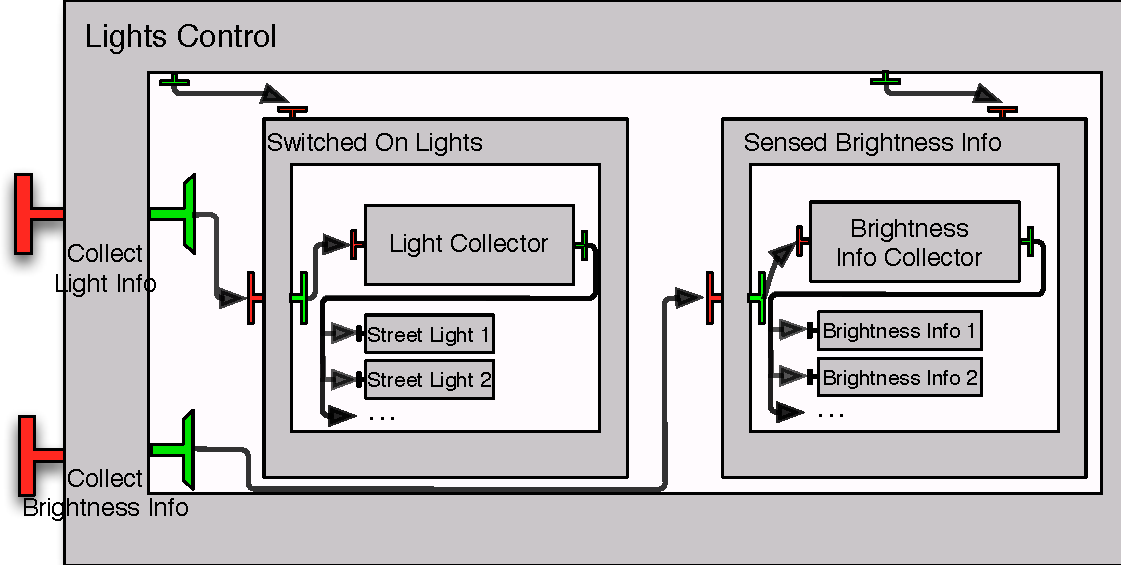
\includegraphics[scale=0.5]{figures/chapter4/usecasearch.pdf} 
   		\caption{Use-Case Architecture}
   		\label{fig:auto}
		\end{figure}

\noindent This use-case consists in an experimental \textsf{component} system 
  in charge of switching on and off street lights, according to the perceived 
  luminosity of the surroundings. Basically, in order to address the goal of
  saving energy, but at the same time offering an acceptable quality of service
  (i.e. an acceptable luminosity in the streets), the \textsf{component}s \textit{Street Light}
  and \textit{Brightness Info} are added/removed accordingly. Moreover, as
 said in \cite{BHN:ICAS09}, the use-case starts with three \textit{Brightness Info}
 \textsf{component}s and zero \textit{Street Light} \textsf{component}. 
  
 We model this scenario in \textsc{Mefresa} by defining every
 \textsf{component} involved in the architecture. For instance, \textsf{component}s
 \textit{Light Collector} and \textit{Street Light} are mechanized as follows:
  
\lstinputlisting[language=Coq]{listings/chapter4/usecase.tex}	
  
  
  \noindent In the above definitions, \textbf{p1} holds the path of 
  both \textsf{component}s in the hierarchy.
  Furthermore, the remaining \textsf{component}s are defined in a similar 
  fashion.  Considering the
  variable \textsf{LightsControlUseCaseArchitecture} as the
  structure holding the complete hierarchy, we can prove its
  well-formedness.
  
\lstinputlisting[language=Coq]{listings/chapter4/usecasearch.tex}	  
  
	\noindent The architecture from this use case indeed meets
	the specification, and proving this lemma poses no particular challenge
	as it has an explicit structure. The interesting aspect of this use-case
	comes from the fact that we need to add and remove \textsf{component}s at runtime.
	Indeed, this scenario is yet another example of the usefulness of being able to
    cope with parametrized specifications.     
    
    
  Before proceeding to the structural reconfigurations, we 
  shall use our \textit{operation} language 
  constructs to define new,
  higher-level constructs. For instance, we can easily define an \textsf{operation}
  to build several \textsf{component}s at a time:
  
  \lstinputlisting[language=Coq]{listings/chapter4/mkcomponents.tex}		
 
\noindent This new \textsf{operation} \textsf{mk\_components} takes
a list of \textsf{component}s as argument and produces a sequence of
\textsf{mk\_component} \textsf{operation}s by means of our 
\textbf{;} constructor. Further, we shall also define an \textsf{operation}
for the construction of a list of \textsf{binding}s.
 
 \lstinputlisting[language=Coq]{listings/chapter4/mkmulticast.tex}

\noindent %As mentioned above, there are three types of bindings -
%\textit{normal}, \textit{import} and \textit{export} -,
%therefore it is natural to imagine three types of multicasts. 

Essentially, it is 
a set of \textsf{binding}s being made from the same client to several
servers. The path \textbf{p} is given as pointer to the \textsf{component} in the hierarchy
where the \textsf{binding} is going to be kept. Then,  we specify the identifiers \textbf{icc}
and \textbf{iic} that determine the \textsf{component} and \textsf{interface} from which the
\textsf{binding} is made from. Since each \textsf{binding} is made to a different \textsf{component},
we need to generate different identifiers. This is achieved in the same manner
as with the \textsf{generate\_from\_template} function defined above: at each
recursion step we suffix \textbf{n} to \textbf{ics} so that we target different \textsf{component}s
for every \textsf{binding} built. Finally, the identifier \textbf{iis} gives the \textsf{interface} to 
which the \textsf{binding} is made to.
 
Having defined our new \textsf{operation}s, we can now proceed to the specification
of the reconfiguration to add \textit{"Street Light"} \textsf{component}s. Below, \textsf{LightComp}
is a variable representing our \textit{"Street Light"} \textsf{component} defined above.
 
\lstinputlisting[language=Coq]{listings/chapter4/usecasereconfig.tex}
 
\noindent Basically, the above creates \textbf{n} \textsf{component}s
by using the \textit{"Street Light"} \textsf{component} as template, and 
then establishes the required \textsf{binding}s. This, could for instance be
used as follows:

\lstinputlisting[language=Coq]{listings/chapter4/usecaseproof.tex}

\noindent Proving the above lemmas is achieved by the same reasoning
techniques as discussed above. Regarding the first lemma, the key ingredient here to note is that
\textsf{component}s are created before establishing the \textsf{binding}s --- and thus
\textsf{binding}s will indeed succeed to be established --- and they are well-formed
since they are generated from a well-formed template \textsf{component}. As such,
reducing this \textsf{operation} to \textbf{Done} is possible. It should be noted that while generalizing
this lemma for \textbf{n} would require a proof by induction, it would still follow the same principle.
As for the second lemma,
it is a natural consequence of our \textit{validity} theorem (see Listing \ref{lst:validity}).



%% @@@@@@@@@@@@
\section{Discussion}
\label{sec:mesfresadiscussion}


	In this chapter we presented a framework to reason
	about the structure of \textsf{GCM} applications mechanized in the Coq Proof Assistant. 
    The main novelty of our approach lies in the use of an \textsf{operation} language
    that allows to build software architectures	that are \textit{correct-by-construction}.
    While we lose some of the automation offered by the usual approach followed by the use of 
	model-checkers, relying on the expressiveness of the Coq Proof Assistant allows us
	to reason on issues that cannot be addressed by usual model-checking techniques.	
	
	The choice of a \textit{deep-embedding} rather than a \textit{shallow} 
	approach for the definition of our  \textsf{operation} language	is also worth discussing.	
	By explicitly using a \textit{datatype} for the encoding of our \textsf{operation} language 
	there is a clear identification of its syntax, letting no doubt on how \textsf{operations} can
	be composed. Further, our goal here is also to formalize the \ac{GCM} specification, a \textit{deep-embedding}
	emphasizes the operational semantics for the building and reconfiguration of architectures. 
		
%	interesting challenges w.r.t. distributed component-based applications structure.
	
	Indeed, the definition of the \ac{GCM} specification in natural language opens
	the door for several interpretations. Further, such a specification is supposed
	to be \textit{flexible} and allow various conceivable implementations. 
	Nevertheless, the \textsc{Mefresa} framework shows that it is possible and fruitful
	to formalize such an undertaking in a proof assistant like Coq.
	Further, is also provides a case-study on the mechanization of \textsf{component} models in
	the context of interactive theorem proving. In fact, the need for such an approach was
	already discussed in \cite{MERLE:2008:INRIA-00338987:1}.
	
	
	%in the Coq Proof Assistant. Our approach differs from the remaining in that we 
	%aim at 
	%providing a semantics that allows the building of  \textit{correct-by-construction} architectures.

	%\paragraph{}
	%adl is the starting point


	%\paragraph{}
	%complementary approach




\chapbreak

	In this chapter we presented \textsc{Mefresa}, a Coq framework for the reasoning on software architectures.
	
		In the following chapter we show its practical facet by demonstrating how we integrated it		
		with the ProActive middleware, and the inherent benefits from this combination.



